\chapter{Esperiments}

\label{ch:experiments}

In this Chapter, we'll use the \texttt{atarieyes} software to test the
effectiveness of the ideas presented in this thesis. The purpose of these
experiments is both to demonstrate that a features extractor can be learnt
with the method proposed, and to show how these features can be used
in combination with the Restraining Bolt for complex RL tasks.

We'll look at two environments: Breakout and Montezuma's Revenge. For the
first we'll test the training process of the features extractor, while the
second is used for a more complete demonstration about the possibilities of
the complete agent (we proceed from learnt features to the application
of the Restraining Bolt).


\section{Breakout}

\label{sec:exp-breakout}

The first environment we'll see is the famous Atari game ``Breakout''.
A frame of this game is shown in Figure~\ref{fig:breakout-frame}.
\begin{figure}
	\centering
	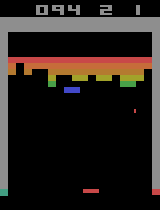
\includegraphics[height=3cm]{./imgs/br1.png}
	\caption{A frame from the Atari game ``Breakout''.}
	\label{fig:breakout-frame}
\end{figure}
The goal is to hit all the bricks with the ball (the small orange dot). Every
time one brick is eliminated, the environment produces a positive reward. The
agent, through the four actions available, \const{NoOp}, \const{Fire},
\const{Right} and \const{Left}, can move the paddle at the bottom and direct
the ball. Every time the paddle misses the ball, the agent loses a life.
However, during training, we terminate and reset the episode at this event.

The exact environment name for this game is \verb|BreakoutDeterministic-v4|.


\subsection{Definitions}

We now define two propositional symbols, \const{Full} and \const{Empty}, and
we apply the proposed model and the training procedure to learn their Boolean
valuation function. The intended interpretation of these two proposition is:
\begin{description}
	\item [\const{Full}] should be true when the area is full of bricks.
	\item [\const{Empty}] should be true when there are no bricks inside the
		area.
\end{description}
The area which we're talking about is shown in
Figure~\ref{fig:breakout-fluents}. The orange rectangle which contains the
intended set of bricks is also the fluents region. So, we've defined two
symbols in one region of the image.
\begin{figure}
	\centering
	\begin{tikzpicture}
		\node [image, tight] (env-br)
			{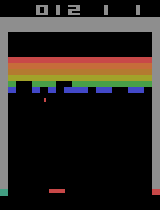
\includegraphics[height=4cm]{./imgs/br2.png}};
		\begin{scope}[shift=(env-br.north west), x={(env-br.north east)},
			y={(env-br.south west)}]
			\draw [region box] \boxblueright node (blueright-coord) {};
		\end{scope}
		\matrix (br-fluents) [right=of env-br,
				matrix of nodes, nodes={anchor=west}] {
			\texttt{full}: true when shot 0 of 18 bricks down \\
			\texttt{empty}: true when shot 18 of 18 bricks down \\
		};
		\draw [->, gray] (br-fluents-1-1.west) to (blueright-coord);
		\draw [->, gray] (br-fluents-2-1.west) to (blueright-coord);
	\end{tikzpicture}
	\caption{In this environment we define two fluents and one region.}
	\label{fig:breakout-fluents}
\end{figure}

How could we \emph{describe the behaviour} of these two propositions with
temporal logic? When an episode starts, we know that \const{Full} should be
true, because all bricks are present, initially. This initial condition is
really helpful. Then, \const{Full} and \const{Empty} represent concepts that
are always mutually exclusive. Finally, since the bricks cannot reappear, we
know that the path is forced: the propositions can't return to a previous
configuration. All these descriptions translate to the following \ldl{}
temporal constraint:
\begin{equation}
	\begin{array}{ll}
		\const{Full}\, \land &
		\to \text{initial condition}\\
		\lbox{\true^*} (\lnot \const{Full} \lor \lnot \const{Empty})\, \land &
		\to \text{exclusive propositions}\\
		\lnot \ldiamond{\true^*; \lnot \const{Full}; \true^*}
		(\const{Full} \land \lnot \lend)\, \land &
		\to \text{can't reappear}\\
		\lnot \ldiamond{\true^*; \const{Empty}; \true^*}
		(\lnot \const{Empty} \land \lnot \lend)\, \land \\
		\lnot \ldiamond{\true^*; \const{Full}} \const{Empty} &
		\to \text{not immediately}\\
	\end{array}
	\label{eq:breakout-constraint}
\end{equation}
The conjunction $\land\, \lnot \lend$ means that we're not referring to the
end of the trace. This is only required in the \ldl{} semantics for finite
traces used here.

The DFA associated to this temporal constraint is shown in
Figure~\ref{fig:breakout-constraint}. This is the automaton that the software
will use to search among the candidate functions.
\begin{figure}
	\centering
	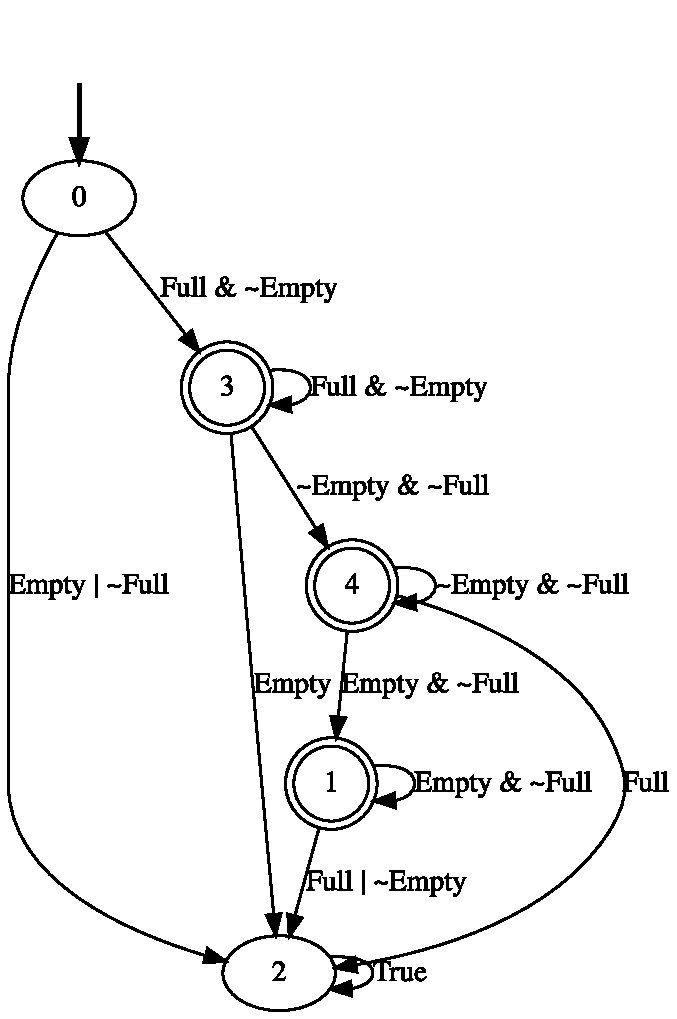
\includegraphics[height=0.5\textheight]{./imgs/br_constraints.pdf}
	\caption{The DFA associated to the formula in
	Equation~\eqref{eq:breakout-constraint}.}
	\label{fig:breakout-constraint}
\end{figure}
As we can see from its structure, the fluents dynamics is relatively simple.
We could have also used the following equivalent formula:
\begin{equation}
	\begin{aligned}
		&\ldiamond{(\const{Full} \land \lnot \const{Empty})^+}
			(\const{End} \,\lor \\
		&\qquad\ldiamond{(\lnot \const{Full} \land \lnot \const{Empty})^+}
			(\const{End} \,\lor \\
		&\qquad\qquad \ldiamond{(\lnot \const{Full} \land \const{Empty})^+}
			\const{End}))
	\end{aligned}
\end{equation}
where the operator $\resym^+$ is an abbreviation of the regular expression
$(\resym; \resym^*)$.

Most states in this automaton are final. In fact, nothing guarantees that the
agent will be able to hit the bricks in every episode. The fluents might not
evolve at all when the agent loses a play.

To specify all these definitions to our software we run:
\begin{minted}{text}
atarieyes features select -e BreakoutDeterministic-v4
\end{minted}
and we select the region of Figure~\ref{fig:breakout-fluents}. Then, we
complete the generated file with the fluents names and any of the two temporal
constraints above. The resulting file is shown in
Listing~\ref{lst:breakout-definitions}. 
\begin{listing}
\begin{minted}{json}
{
  "_frame": [
    8, 32, 152, 197
  ],
	"regions": {
		"blue_right": {
			"abbrev": "br",
			"fluents": [
				"br_full",
				"br_empty"
			],
			"region": [
				32, 87, 152, 93
			]
		}
	},
	"constraints": [
		"br_full",
		"[true*](!br_full | !br_empty)",
		"!<true*; !br_full; true*>(br_full & !end)",
		"!<true*; br_empty; true*>(!br_empty & !end)",
		"!<true*; br_full>br_empty"
	]
}
\end{minted}
\caption{The content of \texttt{definitions/BreakoutDeterministic-v4.json}.}
\label{lst:breakout-definitions}
\end{listing}
"\texttt{br}" is just the abbreviation for that region name. Other than that,
the file exactly represents what we've defined so far.


\subsection{Training}

The first step is to train a RL agent on the environment as it is.
Some of the options we've used for the \verb|agent train| command are: a batch
size of 32, learning rate of $0.0001$, and double Q-Network update every 10000
steps. To follow the training progress, we run TensorBoard on the agent's log
directory.  The results obtained are shown in
Figure~\ref{fig:breakout-agent-train}.
\begin{figure}
	\centering
	\begin{tikzpicture}
		\begin{axis}[
				metrics, xlabel={episode}, ylabel={cumulative reward},
				width=0.7\textwidth, height=0.25\textheight, ymax=90]
			\addplot table
			{./data/run-br-agent-episode_metrics_episode_reward.txt};
		\end{axis}
	\end{tikzpicture}
	\caption{Training the RL agent. Plot of the cumulative reward in each
	episode.}
	\label{fig:breakout-agent-train}
\end{figure}

This plot is the cumulative reward achieved in each episode. At the end of the
training, the agent achieves a reward above 70, which means that is able to
hit 70 bricks without ever losing the ball. This was an expected result,
because at this stage, we just want to replicate the results of previous
studies.  The neural network needs time to adapt to the new observations
reached (a frame without bricks is really different for the Q-Network).
However, we stop this training at 4100 episodes, as this is not the main
purpose of this experiment. These performances are, in fact, sufficient to
reach states in which \const{Empty} becomes true. So, we're ready to train the
features extractor.

The fluents are trained from a dataset generated online by a running agent.
So, we start the trained agent from the previous step:
\begin{minted}[escapeinside=“”]{text}
atarieyes agent play “\normalfont<args-file>” -c “\normalfont<checkpoint>” --rand-test 0.1
\end{minted}
where <checkpoint> is any saved agent from the previous training. When
training the feature extractor, the agent should avoid repetitive behaviours,
and try to thoroughly explore the environment. This command selects a
0.1-greedy policy, but we've also experimented with many others, such as
\verb|--rand-eps|. We let this command run and focus on the receiving side.

The network that we use for the encoder is a DBN of size $(N, 50, 20)$. $N$ is
the number of input pixels in our region, but this is computed by the
software and we don't need to specify it. This network contains two RBMs and
generates an encoding of 20 binary units. At first sight, this encoding could
seem quite large. However, we must consider that there are 18 bricks in the
selected region. If we want to learn a representation for these bricks, there
must be at least 18 units. 20 constitutes a nearly-optimal size for this
encoding (we use 20, because the optimal might not be reachable during
training). Also, we've observed that the shallow network $(N, 20)$ is not able
to achieve the same performances as the deep architecture selected here.

First, we train the layer number~0, that is of size $(N, 50)$, with the
following command:
\begin{minted}{bash}
atarieyes features train --network 50 20 --train blue_right 0
\end{minted}
Other omitted arguments are: the environment, learning rate of $0.001$,
batch size of 50 and regularization factors.

The output of this training is shown by the plots on the left in
Figure~\ref{fig:plot-br-encoder}. The most important is the free energy, shown
in the top left plot, that we've defined in Equation~\eqref{eq:free-energy} at
page~\pageref{eq:free-energy}. A low free energy means that the model is
recognizing the training dataset, because a low energy is associated to a high
probability for the input batches. The second metric, the reconstruction
error, shows the $L_1$ distance between the input images and the reconstructed
images (reconstructions are the most probable images under the encoding
assigned for the true inputs). Minimizing the reconstruction error is not the
training objective of Persistent CD, but it's useful to visualize it anyway,
because, unlike the free energy, we know its correct scale and lower bound.

\begin{figure}[p]
	\hspace*{-2cm}%
	\begin{minipage}{\textwidth+3.5cm}
	\begin{tikzpicture}
		\pgfplotsset{
			every axis/.append style={
				metrics, width=0.4\textwidth, height=0.25\textheight,
				enlarge x limits=false,
			}
		}
		\begin{axis} [
				name=free energy 0, xlabel={step}, ylabel={free energy}]
			\addplot table
			{./data/run-br-features-logs0-metrics_free_energy.txt};
		\end{axis}
		\begin{axis}[
				at=(free energy 0.below south), anchor=above north,
				xlabel={step}, ylabel={reconstruction error}, ymin=0, ymax=0.5]
			\addplot table
			{./data/run-br-features-logs0-metrics_reconstruction_error.txt};
		\end{axis}
		\begin{axis} [
				name=free energy 1,
				at=(free energy 0.right of east), anchor=left of west,
				xlabel={step}]
			\addplot table
			{./data/run-br-features-logs2-metrics_free_energy.txt};
		\end{axis}
		\begin{axis}[
				at=(free energy 1.below south), anchor=above north,
				xlabel={step}, ymin=0, ymax=0.5]
			\addplot table
			{./data/run-br-features-logs2-metrics_reconstruction_error.txt};
		\end{axis}
		% Titles
		\node [above, yshift=3ex] at (free energy 0.above north)
			{Training layer 0 -- $(N, 50)$};
		\node [above, yshift=3ex] at (free energy 1.above north)
			{Training layer 1 -- $(50, 20)$};
	\end{tikzpicture}
	\caption{Training metrics of the encoder model.}
	\label{fig:plot-br-encoder}
	\end{minipage}%
	\hspace*{-1.5cm}%
\end{figure}

We can also appreciate the trained model, by looking at the quality of its
reconstructions. The top row of Figure~\ref{fig:imgs-br-encoder-0} shows three
input images in our region. Each of these inputs has a different
configuration of bricks. On the bottom row, we see the expected input images,
given the encoding that the model associates to the inputs above\footnote{ The
expected input has a likelihood term, that is generated from the encoding, and
a prior expectation, which derives from the most frequent input patterns. So,
the expected input is a probabilistic prediction and it shouldn't be properly
considered an input reconstruction.  }.

\begin{figure}
	\centering
	\begin{tikzpicture}
		\matrix [
			matrix of nodes, nodes={image, tight, draw, thin},
			row sep=4mm, column sep=6mm, outer sep=3mm,
		] {
			
\includegraphics[width=4cm]{./imgs/br_encoder_layer0_last_true.png} \&
			
\includegraphics[width=4cm]{./imgs/br_encoder_layer0_last1_true.png} \&
			
\includegraphics[width=4cm]{./imgs/br_encoder_layer0_last2_true.png} \\
			
\includegraphics[width=4cm]{./imgs/br_encoder_layer0_last_est.png} \&
			
\includegraphics[width=4cm]{./imgs/br_encoder_layer0_last1_est.png} \&
			
\includegraphics[width=4cm]{./imgs/br_encoder_layer0_last2_est.png} \\
		};
	\end{tikzpicture}
	\caption{True inputs (top row) and expected input images (bottom row).
	Reconstructions generated with layer~0.}
	\label{fig:imgs-br-encoder-0}
\end{figure}

Now that the first layer is trained correctly, we proceed to the second and
final layer of this encoder. With the commands \verb|--train| and
\verb|--init| we can train the next layer (the index is 1) from the weights
obtained at the previous step. The results are shown in the right-hand column
of Figure~\ref{fig:plot-br-encoder}. We have now trained an encoder that
transforms the input image for this region in a vector of 20 binary units.

Since this is the only encoder, we can now pass to discuss the Boolean
functions. To train this final ``layer'', we issue a similar command:
\begin{minted}{bash}
atarieyes features train --network 50 20 --train all 2
\end{minted}
For the moment, let's ignore the specific parameters used in this case. We can
directly look at the training outcome in the plots of
Figure~\ref{fig:plot-br-bool}.
\begin{figure}[p]
	\centering
	\begin{tikzpicture}
		\pgfplotsset{
			every axis/.append style={
				metrics, width=0.8\textwidth, height=0.25\textheight,
				/pgfplots/.cd,
				minor xtick={90,223,263}, grid=none, xminorgrids,
			},
		}
		\begin{axis}[
				name=consistency, xlabel={step}, ylabel={avg. consistency},
				/pgfplots/table/.cd, col sep=comma, x=step, y=consistency,
			]
			\addplot table {./data/run-br-features-logs5-metrics.txt};
			\addplot table {./data/run-br-features-logs6-metrics.txt};
			\addplot table {./data/run-br-features-logs7-metrics.txt};
			\addplot table {./data/run-br-features-logs8-metrics.txt};
		\end{axis}
		\begin{axis}[
				name=sensitivity, xlabel={step}, ylabel={avg. sensitivity},
				at=(consistency.below south), anchor=above north, yshift=-0.5cm,
				/pgfplots/table/.cd, col sep=comma, x=step, y=sensitivity,
			]
			\addplot table {./data/run-br-features-logs5-metrics.txt};
			\addplot table {./data/run-br-features-logs6-metrics.txt};
			\addplot table {./data/run-br-features-logs7-metrics.txt};
			\addplot table {./data/run-br-features-logs8-metrics.txt};
		\end{axis}
		\begin{axis}[
				name=fitness, xlabel={step}, ylabel={avg. fitness},
				at=(sensitivity.below south), anchor=above north, yshift=-0.5cm,
				/pgfplots/table/.cd, col sep=comma, x=step, y=fitness,
			]
			\addplot table {./data/run-br-features-logs5-metrics.txt};
			\addplot table {./data/run-br-features-logs6-metrics.txt};
			\addplot table {./data/run-br-features-logs7-metrics.txt};
			\addplot table {./data/run-br-features-logs8-metrics.txt};
		\end{axis}
	\end{tikzpicture}
	\caption{Training metrics generated by the GA for the Boolean functions:
	population average values for consistency, sensitivity and fitness.}
	\label{fig:plot-br-bool}
\end{figure}
From top to bottom, they show the values of ``consistency'', ``sensitivity''
and fitness, averaged over all candidate functions. These metrics are computed
with respect to the automaton in Figure~\ref{fig:breakout-constraint}. Only
the fitness value contributes to the reproduction probability of each
individual. The other two metrics are shown just to get a better
understanding.

As we can see from the first peak in the consistency plot, the genetic
algorithm, just by eliminating all the candidates that do not predict
$\set{\const{Full}}$ for the initial configuration, is able to be consistent
with the constraint. Then, to further improve the fitness, the algorithm
looks for functions that are also able to explore the automaton states. Of
course, this comes at a risk of falling into rejecting states.
It seems that better candidates are found at step 220 and 260, where
predictions visit all the automaton final states, always satisfying the
constraint, at the end of the trace.

The colors and the vertical lines in Figure~\ref{fig:plot-br-bool} separate
different training commands. After each interruption we resume from the
previous state with the \verb|--cont| option. This detail is relevant because,
as training progresses, the most appropriate hyper-parameters change. From
left to right, the algorithm parameters for each run are the following:
\begin{center}
\begin{tabular}{l*4c}
	\texttt{--fitness-episodes} & 2 & 5 & 12 & 20 \\
	\texttt{--fitness} & (30, 100) & (30, 100) & (10, 100) & (10, 100) \\
	\texttt{--mutation-p} & 0.02 & 0.02 & 0.005 & 0.002 \\
	\texttt{--crossover-p} & 0.02 & 0.02 & 0.005 & 0.002
\end{tabular}
\end{center}
The most important is \texttt{--fitness-episodes}, which determines how many
episodes are observed in order to compute the fitness function. As training
progresses, we should increase this number, because the target function should
be ideally consistent with any trace. A good nondeterminism from the agent's
side, helps to generate diverse test episodes and to keep this number limited.
Similarly, the other parameters follow a similar idea: training should slow
down and be more accurate over time.  At the end of this process, a best
candidate is selected according to the criterion described in the previous
chapter: the individual with maximum consistency and highest sensitivity.


\subsection{Comments}

We've now trained a complete features extractor. From an image of the Breakout
environment, it's able to predict a Boolean value for \const{Full} and
\const{Empty}. To verify the quality of the result, we can just make
predictions with this model. We can see few predictions in
Figure~\ref{fig:breakout-predict}. For compactness, we show just a portion of
the entire frame, and the input region is highlighted in the rectangle.
\tikzset{
	image part/.style={path picture={
		\node (#1) [image, tight]
			at ($(path picture bounding box.center)+(0,-0.5cm)$)
			{\includegraphics[height=4cm]{./imgs/#1.png}};
		\begin{scope}[shift=(#1.north west), x={(#1.north east)},
				y={(#1.south west)}]
			\draw [region box] \boxblueright node (blueright-coord) {};
		\end{scope}
	}},
	draw image part/.code={
		\begin{scope}[yshift=-0.6cm]
			\path [image part=#1, rounded corners]
				rectangle (3cm,1.2cm) [sharp corners];
		\end{scope}
	},
}
\begin{figure}
	\centering
	\begin{tikzpicture}
		\matrix [row sep=4pt, column sep=0.4cm] {
			\node [right, xshift=0.4cm] {\footnotesize input images}; \&
			\node {\const{Full}}; \& \node {\const{Empty}}; \\[10pt]
			\tikzset{draw image part=br0} \& \node {T}; \& \node {F}; \\
			\tikzset{draw image part=br2} \& \node {F}; \& \node {F}; \\
			\tikzset{draw image part=br1} \& \node {F}; \& \node {F}; \\
			\tikzset{draw image part=br3} \& \node {F}; \& \node {T}; \\
		};
	\end{tikzpicture}
	\caption{Predictions on Breakout with the trained model.}
	\label{fig:breakout-predict}
\end{figure}

In these, and many more cases that we tested, the model is always correct. The
only wrong prediction we could find is the following:
\begin{center}
	\begin{tikzpicture}
		\matrix [column sep=0.4cm] {
			\& \node {\const{Full}}; \& \node {\const{Empty}}; \\
			\tikzset{draw image part=br4} \& \node {T}; \& \node {F}; \\
		};
	\end{tikzpicture}
\end{center}
where it mistakenly predicts that the region is still full of bricks. To
understand this small error, we looked at the agent's plays and we discovered
that it has learnt to always hit that brick at the very first touch with the
ball. Let's see what this repetitive behaviour had caused.

One great advantage of working with Boolean functions from a compact encoding
space is that we can inspect and understand what the model has learnt to
recognize; i.e. which input patterns the model associates to a true output. To
do so, we need to visualize both the meaning of the Boolean features and the
Boolean rules deciding from such features.

\begin{figure}[tb]
	\centering
	\begin{tikzpicture}
		\node [image, tight] (bars) {
			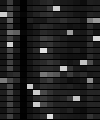
\includegraphics[width=7cm,interpolate=false]{./imgs/br_model_all.png}};
		\matrix [
			matrix of nodes, nodes in empty cells,
			right=1cm of bars.north east, anchor=north west, tight,
			row sep={4.22mm,between origins}, column sep=1cm,
		] (rules) {
			 0\&      1\\   
			 1\&      0\\   
			 1\&     \\   
			\&        0\\   
			\&       \\   
			 1\&     \\   
			 1\&     \\   
			\&       \\   
			\&        0\\   
			 0\&      1\\   
			 1\&     \\   
			\&        0\\   
			\&       \\   
			\&        0\\   
			\&        0\\   
			\&        0\\   
			 1\&     \\   
			\&       \\   
			\&        1\\   
			\&        0\\   
		};
		\matrix [
			matrix of nodes, nodes in empty cells,
			left=1cm of bars.north west, anchor=north east, tight,
			row sep={4.22mm,between origins}, column sep=1cm,
		] (numbers) {
			1\\2\\3\\4\\5\\6\\7\\8\\9\\10\\11\\12\\13\\14\\15\\16\\17\\18\\19\\20\\
		};
		\matrix [above=0.4cm of rules, matrix of nodes] {
			\texttt{full} \& \texttt{empty} \\
			1-rule \& 1-rule \\
		};
		\node [above=0.7cm of bars] {expected input per unit};
		\node [above=0.7cm of numbers] {encoding units};
	\end{tikzpicture}
	\caption{Visualization of the trained encoder and Boolean functions. Each
	row represents an input feature. Details are explained in the main text.}
	\label{fig:breakout-model-all}
\end{figure}
The large image in Figure~\ref{fig:breakout-model-all} contains 20 ``rows''.
The $i$-th row in this image is the \emph{expected input} region that the DBN
predicts, given an encoding vector of zeros except for a 1 at the $i$-th
position (we can do this backpropagation because the encoder is a
probabilistic model). So, each line contains the input that is most
correlated with each encoding unit; essentially, what each unit represents.
It emerges an interesting result: each unit is correlated to the presence of
one, or at most two bricks. For example, when the left-most brick is present,
the third unit of the encoder is~1, and vice versa.

The most probable inputs shown here are also affected by a prior probability.
In fact, the fourth brick, which is almost always down, is the same that the
agent has learnt to hit first (see the dark column). Since the fourth brick is
so rare, the model didn't associate any unit to its precence, but it has only
assigned a strong prior probability, instead. So, the wrong prediction we've
seen above is caused by a too coarse encoding. Clearly, everything that the
encoder considers of the same class cannot be distinguished by the Boolean
functions.

On the right of Figure~\ref{fig:breakout-model-all}, there are two columns of
0s and 1s.  These are the Boolean rules (1-rules) of the best candidate that
the model has selected. We can recognize a reasonable pattern: the rule for
\const{Full} requires the absence of the features 1 and 10, which detect the
empty line, and the presence of many other features, which are associated to
the presence of each brick. The rule for \const{Empty} does almost the
opposite.

We also understand that the concept for \const{Full} is not learnt exactly,
because the rule doesn't require anything about the second brick (feature
number 8). This is not necessarily an error: we want the features extractor to
give correct valuations just for the trajectories visited by the agent, not
for any input. In fact, the training dataset are the observations produced by
the agent, and we want the valuations function to be correct on those. In this
example, the light colour of the second column suggests that the second brick
is the last to be hit. At that point, the model has many other evidences that
\const{Full} must be false (other bricks required by the rule are down,
already). So, it didn't need to link the concept of the fluent to the 8th
feature. In general, this is the reason why the agent's policy should have a
strong stochastic component: to encounter as many possible trajectories during
the training phase.

To conclude, this game is not considered a complex environment for Deep RL,
because it has been solved as one of the first games. Instead, it can be a
much more challenging environment, if we consider the features extraction
problem. The difficulty of learning some propositions doesn't reside in the
cumulative reward, but on the complexity of the observations and on the
desired meaning of the propositions. This problem quickly becomes hard when
we want to learn very complex concepts.

Even though our observations had very little noise (the ball passing was the
only noise, in fact), we selected a region with many meaningful
configurations. Due to the combinatory nature of the bricks, we've asked the
features extractor to detect one in $2^{18}$ configurations, which is not an
easy task. As we've seen, this goal as been achieved almost perfectly.

Due to the way temporal constrains and metrics work, it's better to learn some
correlated fluents at the same time. Even if we would only need \const{Full}
for some temporal goal, we wouldn't be able to learn one of the two symbols in
isolation.


\section{Montezuma's Revenge}

With the previous game, we've shown that it's indeed possible to learn Boolean
propositions of moderate complexity. Here, instead, we demonstrate the
complete training procedure described in
Section~\ref{sec:training-incremental}: from a completely inexpert agent,
we'll obtain a capable one, that bases its decisions on the features learnt.

We'll use a second game from the Atari collection, called Montezuma's Revenge
(the precise environment name is
\verb|MontezumaRevengeDeterministic-v4|). Figure~\ref{fig:mz-frame} shows the
initial image of this game.
\begin{figure}
	\centering
	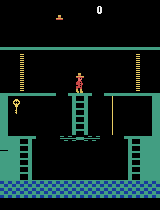
\includegraphics[height=4cm]{./imgs/mz0.png}
	\caption{A frame from the Atari game ``Montezuma's Revenge''.}
	\label{fig:mz-frame}
\end{figure}
The agent's goal is to move the character inside the many rooms of the
labyrinth, collect the items required to advance, and avoid enemies. The
action space is composed by 18 actions. They allow to move the agent to remain
still, move left-right, up-down (and combinations of the two), optionally
while performing the \texttt{fire} action.

As we can imagine from the many actions and the more complex map, this game is
much harder for a RL agent with respect to Breakout. In fact, it's
arguably the most difficult among all games in the Atari~2600 collection. We
can see, for example, that in~\cite{bib:atari-deepq-nature} the DQN agent
achieves no rewards at all. This difficulty arise from two factors: partial
observations (because of the many rooms), and sparse rewards. Luckily, both
issues can be addressed with the Restraining Bolt, because it can be used to
provide additional rewards when specific trajectories or simple conditions are
reached.


\subsection{Definitions}

The problem of sparse rewards is the first difficulty the agent faces. In
fact, reaching the first rewarded state, which is taking the key of
Figure~\ref{fig:mz-frame}, requires a long sequence of correct actions that is
almost impossible to achieve at random.

The fluents that we'll define serve for this purpose: correctly navigating
this first room. Four of them, \const{AtStart}, \const{AtStairs1},
\const{AtStairs1bot}, \const{AtStairs2}, should be valuated to true if the
character is at each of these positions. We can see the regions to which they
refer, in Figure~\ref{fig:mz-fluent-regions}. The last one, \const{KeyTook},
should be true when the key has been taken by the agent.

\begin{figure}
	\centering
	\begin{tikzpicture}
		\node (frame) [image, tight]
			{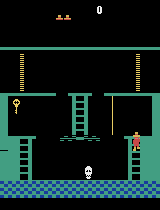
\includegraphics[height=7cm]{./imgs/mz2.png}};
		\begin{scope}[shift=(frame.north west),
				x={(frame.north east)}, y={(frame.south west)},
				every node/.append style={circle, tight, minimum size=15pt}
			]
			\draw [region box] \boxstart node (start pos) [pos=0.5] {};
			\draw [region box] \boxstairsone node (stairs1 pos) [pos=0.5] {};
			\draw [region box] \boxstairsonebot node (stairs1bot pos) [pos=0.5] {};
			\draw [region box] \boxstairstwo node (stairs2 pos) [pos=0.5] {};
			\draw [region box] \boxkey node (key pos) [pos=0.5] {};
		\end{scope}
		\coordinate (frame east) at ($(frame.east)+(0.5cm,0)$);
		\coordinate (frame west) at ($(frame.west)+(-0.5cm,0)$);
		\path [<-, draw=white, double=black] (start pos) -- (frame east |- start pos) node [right] {\const{AtStart}};
		\path [<-, draw=white, double=black] (stairs1 pos) -- (frame east |- stairs1 pos) node [right] {\const{AtStairs1}};
		\path [<-, draw=white, double=black] (stairs1bot pos) -- (frame east |- stairs1bot pos) node [right] {\const{AtStairs1bot}};
		\path [<-, draw=white, double=black] (stairs2 pos) -- (frame west |- stairs2 pos) node [left] {\const{AtStairs2}};
		\path [<-, draw=white, double=black] (key pos) -- (frame west |- key pos) node [left] {\const{KeyTook}};
	\end{tikzpicture}
	\caption{Definition of five fluents and their associated regions. The
	correct valuation for this frame would be: $\set{\const{AtStairs1}}$.}
	\label{fig:mz-fluent-regions}
\end{figure}

We can clearly use these symbols to guide the agent through the room,
rewarding it at each spot reached. When it grabs the key, the environment
sends a reward, so that of the RB is redundant. However, in order to progress,
the agent has to get the key and come back to the start position. So,
\const{KeyTook} is required in order to write the correct temporal
specification.

As we've seen in Section~\ref{sec:training-incremental}
``\nameref{sec:training-incremental}'', we can't directly learn the fluents
that the agent is not able to influence. In this case, we can't learn what it
means \const{KeyTook} until the agent is able to grab it. So, only
\const{AtStart} and \const{AtStairs1} will be learnt, initially. Then, every
time the agent becomes able to reach a new position, we can expand our
definitions to include a new symbol to learn.

We'll now show the complete JSON file of definitions, but, for brevity, we'll
omit the symbol \const{AtStairs1bot}. The file is shown in
Listing~\ref{lst:mz-definitions}. The \texttt{restraining\_bolt} section is
empty here, but it will be filled later on.
\begin{listing}
\begin{minted}{json}
{
  "_frame": [ 0, 47, 160, 180 ],
  "regions": {
    "start": {
      "abbrev": "start",
      "region": [ 74, 79, 87, 87 ],
      "fluents": ["start_at"]
    },
    "stairs1": {
      "abbrev": "stairs1",
      "region": [ 131, 129, 141, 145 ],
      "fluents": ["stairs1_at"]
    },
    "stairs2": {
      "abbrev": "stairs2",
      "region": [ 19, 167, 29, 181 ],
      "fluents": ["stairs2_at"]
    },
    "key0": {
      "abbrev": "key0",
      "region": [ 11, 98, 22, 116 ],
      "fluents": ["key0_took"]
    }
  },
  "constraints": [
		"start_at & !key0_took",
		"[true*](start_at -> !(stairs1_at | stairs2_at))",
		"[true*](stairs1_at -> !(start_at | stairs2_at))",
		"[true*](stairs2_at -> !(start_at | stairs1_at))",
		"[true*; start_at]!(stairs1_at | stairs2_at)",
		"[true*; stairs1_at]!(start_at | stairs2_at)",
		"[true*; stairs2_at]!(start_at | stairs1_at)"
	],
  "restraining_bolt": []
}
\end{minted}
\caption{The content of \texttt{definitions/BreakoutDeterministic-v4.json}
(symbol \texttt{stairs1bot\_at} omitted for brevity).}
\label{lst:mz-definitions}
\end{listing}
Other than the initial condition, this constraint states that the
``\const{At}'' propositions are mutually exclusive, because the agent can be
only in one place at the time. Also, at least one instant is needed to pass
from one place to the other.


\subsection{Training}

Following the same procedure as in the previous game, we should train the RL
agent alone on the environment rewards. However, as previously studies had
found, the agent can't reach any reward at all, here. This is fine. The first
agent is used just to train the features extractor. The random policy will be
enough to learn the first two symbols: \const{AtStart} and \const{AtStairs1}.
So, we run:
\begin{minted}[escapeinside=“”]{text}
atarieyes agent play “\normalfont<args-file>” -c “\normalfont<checkpoint>” --rand-test 1
\end{minted}
which plays completely with random actions.

The encoder network we chose is a DBN with size $(N, 10, 1)$. This means that
each input region is encoded into a single Boolean value. Let's discuss this
choice: a scalar encoding means that the fluent value will be exactly the
extracted Boolean feature. Therefore, the Boolean functions play no role at
all in the selection of the desired concept (they can only negate the received
value).  This is intentional. As we've previously noted, the encoding size
should be the smallest number of units that are sufficient to determine the
truth of the propositions. If, with a single unit, the encoder is able to
isolate the required feature by itself, there's no point in transfering this
task to the Boolean functions, where the separation might be more complex.

The training command for the first layer of the encoder at the ``start''
region is:
\begin{minted}{bash}
atarieyes features train --network 10 1 --train start 0
\end{minted}
We repeat this process for layer~1 and the encoder at region ``stairs1''.
All these runs are much faster than in the Breakout case, because the
input images show little diversity. On the other end, the event we're trying
to catch is very rare (the agent needs to pass on each region by chance), so
we use a slightly larger batch size, with~100 images.
Figure~\ref{fig:plot-mz-encoder} shows the reconstruction error for each of
these four trainings. We omit plots for the last layer, the Boolean functions.

\begin{figure}[p]
	\centering
	\begin{tikzpicture}
		\pgfplotsset{
			every axis/.append style={
				metrics, width=0.7\textwidth, height=0.18\textheight, ymin=0,
			},
			/pgfplots/table/.cd, col sep=comma, x=Step, y=Value,
		}
		\begin{axis} [
				name=run0, ylabel={layer (start, 0)},
			]
			\addplot table
				{./data/run-mz-features-logs0-metrics_reconstruction_error.csv};
		\end{axis}
		\begin{axis} [
				name=run1, at=(run0.below south), anchor=above north, yshift=-0.5cm,
				ylabel={layer (start, 1)},
			]
			\addplot table
				{./data/run-mz-features-logs1-metrics_reconstruction_error.csv};
		\end{axis}
		\begin{axis} [
				name=run2, at=(run1.below south), anchor=above north, yshift=-0.5cm,
				ylabel={layer (stairs1, 0)},
			]
			\addplot table
				{./data/run-mz-features-logs2-metrics_reconstruction_error.csv};
		\end{axis}
		\begin{axis} [
				name=run3, at=(run2.below south), anchor=above north, yshift=-0.5cm,
				xlabel={step}, ylabel={layer (stairs1, 1)},
			]
			\addplot table
				{./data/run-mz-features-logs3-metrics_reconstruction_error.csv};
		\end{axis}
	\end{tikzpicture}
	\caption{Training metric for each encoder and layer. The x-axis is the
	training step, the y-axis is the reconstruction error.}
	\label{fig:plot-mz-encoder}
\end{figure}

The features extractor obtained correctly valuates both symbols,
\const{AtStart} and \const{AtStairs1}, in all images that we tested. Let's see
what the model has learnt. In Figure~\ref{fig:mz-expected-inputs}, we
visualize the expected input images given the output encodings, in a similar
way to Figure~\ref{fig:breakout-model-all}. In this case, the encoding is
composed of just one Boolean unit. So, we show the input associated to both
values.
\begin{figure}
	\centering
	\begin{tikzpicture}[img box/.style={image, draw, thick}]
		\matrix [row sep=0.5cm, column sep=0.5cm] {
			\& \node {encoding~0}; \& \node {encoding~1}; \\
			\node {``start''\\region}; \&
			\node [img box] {
\includegraphics[width=3cm]{./imgs/mz_start_0.png}}; \&
			\node [img box] {
\includegraphics[width=3cm]{./imgs/mz_start_1.png}}; \\
			\node {``stairs1''\\region}; \&
			\node [img box] {
\includegraphics[height=3.5cm]{./imgs/mz_stairs_0.png}}; \&
			\node [img box] {
\includegraphics[height=3.5cm]{./imgs/mz_stairs_1.png}}; \\
		};
	\end{tikzpicture}
	\caption{Expected input images for each region and encoding output.
	The differences between columns have been emphasized.}
	\label{fig:mz-expected-inputs}
\end{figure}

The left images are the expected inputs when the encodings are~0, while
the right are associated to~1. Since the character is rarely inside the
regions, there is a strong bias that tend to uniform all these images. So,
we've slightly emphasized the differences between the two columns to improve
this visualization. As we can now understand, the encoders have learnt to
recognize when the agent is \emph{not} inside each region. The slight gray
tones in the left column mean that there is some possibility for the agent to
be there, when the encoding is~0; while it is certainly not there for the
output~1. In fact, if we then look at the Boolean rules, we would see that
this encoding is negated to produce the fluent valuations.

The now complete features extractor can be used to guide the agent with
additional rewards. We write the following simple temporal goal:
\begin{equation}
	\ldiamond{(\lnot \const{AtStairs1})^*}(\const{AtStairs1} \land \llast)
\end{equation}
which sends a single reward when the agent reaches the stairs on the right
(see the regions in Figure~\ref{fig:mz-fluent-regions}). We write this formula
on the field \texttt{restraining\_bolt} in the file of definitions. If we
remember that the agent wasn't able to reach any reward at all, this initial
goal is a way to start.

We now train the RL agent on this goal by executing both \verb|agent train|
and \verb|features rb|. Once we see that the agent has learnt to reach this
first goal, we can repeat the previous process for a new symbol. In this case,
we would let the trained agent play, and train the features extractor for the
symbol \const{AtStairs1bot}, which is the next encountered the path.  With
this iterative procedure we've been also able to learn \const{AtStairs2}.

To this point, we've mainly addressed the problem of sparse rewards, because
the Restraining Bolt has been used to send rewards upon the detection of some
events.  However, we can also use it to solve non-Markovian tasks.
Suppose we want the agent to repeatedly jump from ``start'' to ``stairs1'' and
vice versa. This apparently simple problem cannot be solved just providing the
appropriate rewards, because, from one input frame, the policy hasn't
enough information about where to direct the player. Instead, the RB is able
to provide a consistent information about the next position to reach.

In the \verb|restraining_bolt| field, we now write a \ldl{} formula, that,
combined with the temporal constraints, corresponds to the automaton in
Figure~\ref{fig:mz-repetitive-goal-automa}.
\begin{figure}
	\centering
	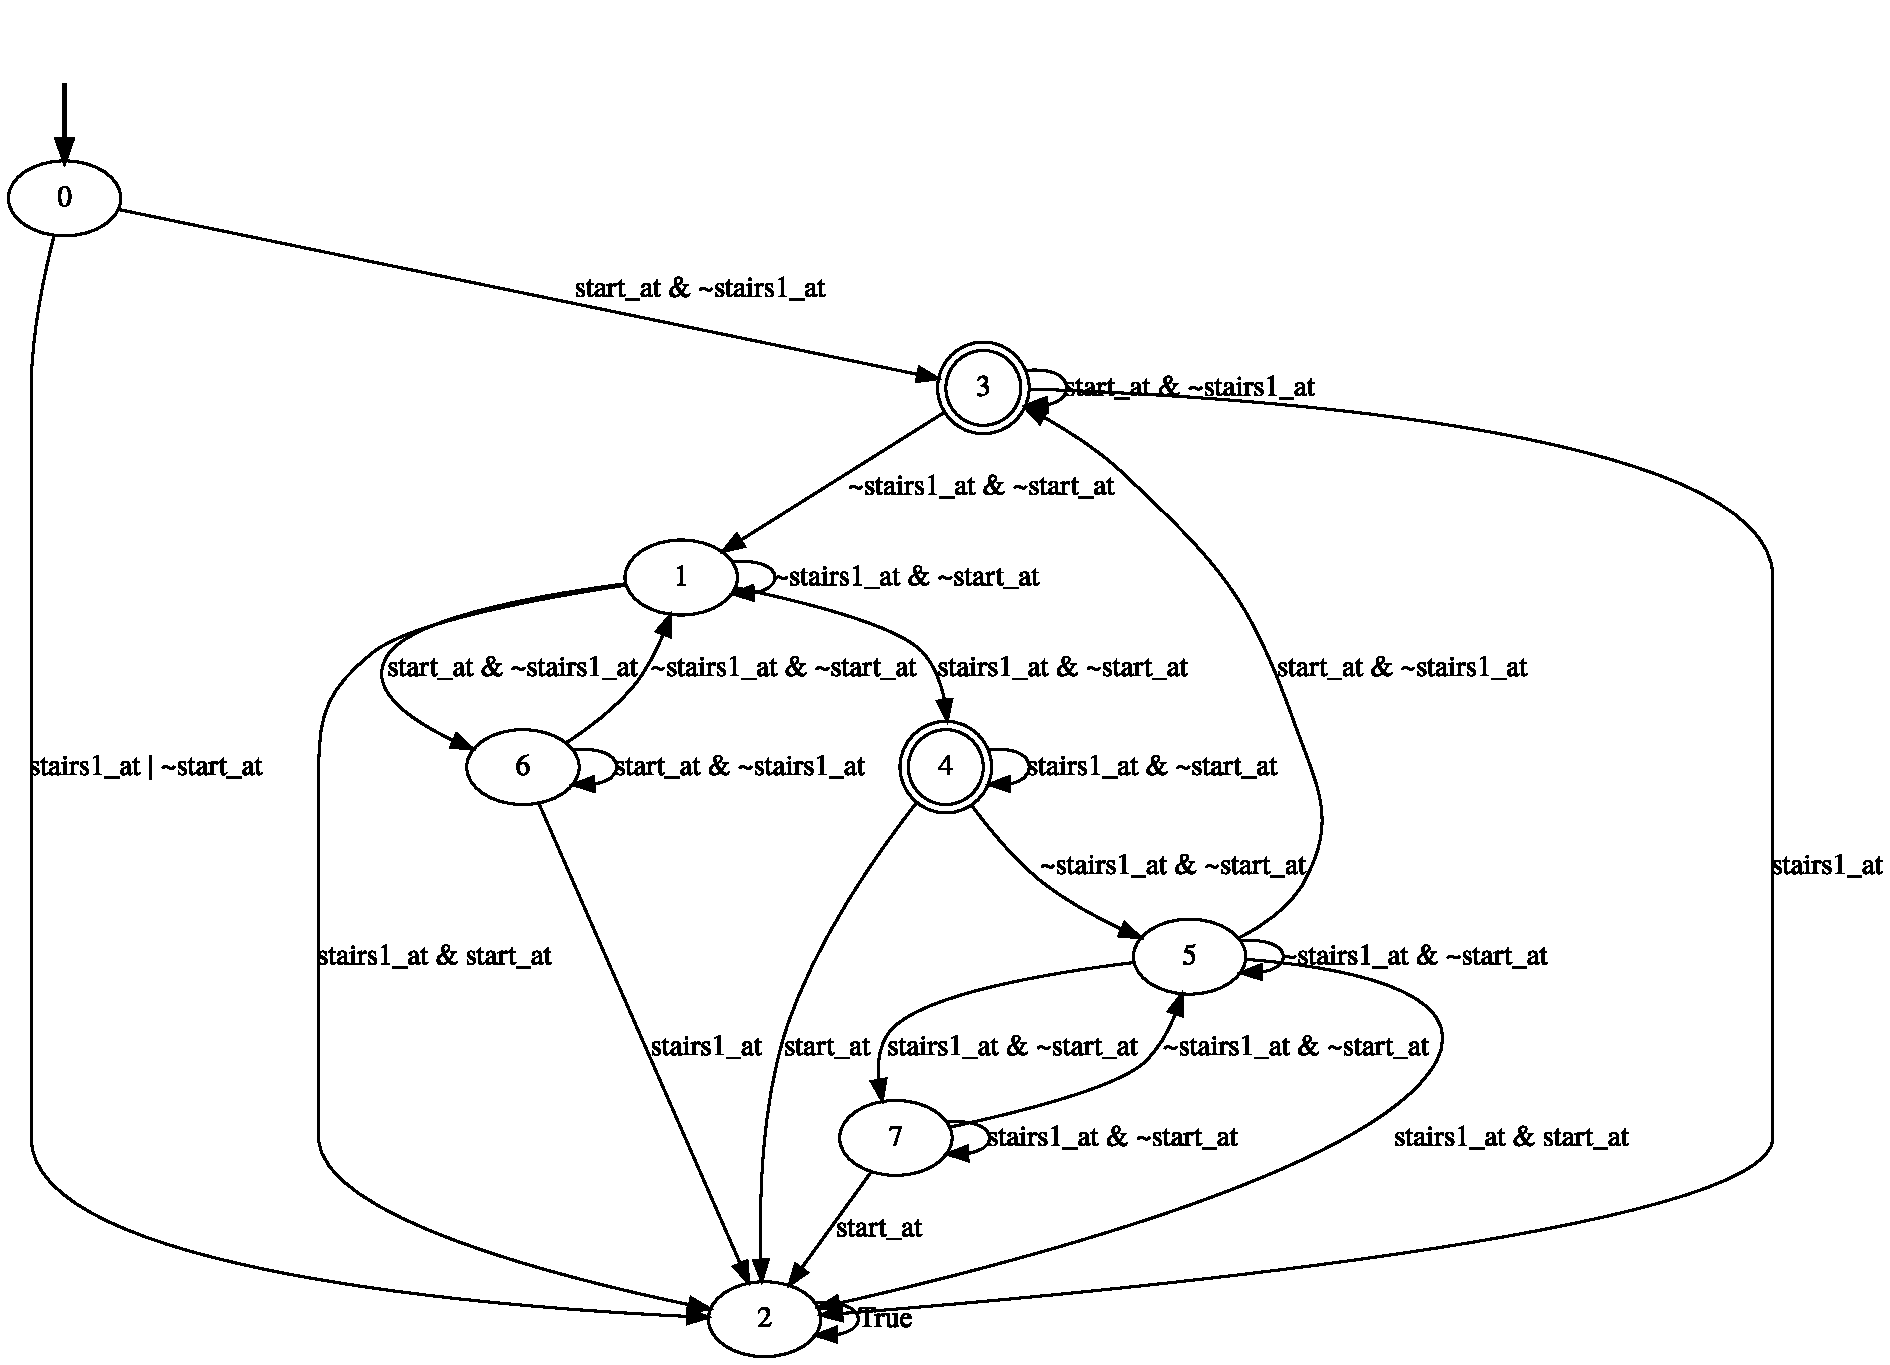
\includegraphics[width=\textwidth]{./imgs/mz-repetitive-goal-automa.pdf}
	\caption{Automaton associated to the last temporal goal (back and forth from
	``start'' to ``stairs1'').}.
	\label{fig:mz-repetitive-goal-automa}
\end{figure}
What this specification says is that the agent can accumulate rewards,
represented by the final states, by following the cycle of states: ${3 \to}\,
1 \to 4 \to 5\, {\to 3}$. So, it is induced to pass from ``start'' to
``stairs1'' and vice-versa. This is only possible, because the agent also
receives from the RB in which of these states it is.

Seen as an image-to-action function, the agent's policy corresponding to
states 4, 7 and 5 will tend toward the position ``start'', while for 1, 6 and
4, it will point in the opposite direction. We run the usual
\texttt{agent}--\texttt{features} pair of instances to train the agent on this
new goal. In Figure~\ref{fig:mz-repetitive-goal-reward}, we show the
the cumulative reward during this training.
\begin{figure}
	\centering
	\begin{tikzpicture}
		\begin{axis}[
				metrics, xlabel={eposode}, ylabel={cumulative reward},
				width=0.7\textwidth, height=0.2\textheight,
				xmin=3403, ymin=0, enlarge x limits=false, ymax=15]
			\addplot table
				{./data/run-mz-agent-repetitive-reward.txt};
		\end{axis}
	\end{tikzpicture}
	\caption{Training the RL agent on the ``start''--``stairs1'' goal. Plot of
	the cumulative reward in each episode.}
	\label{fig:mz-repetitive-goal-reward}
\end{figure}
The increase we see means that the agent is learning to get from one position
to the other, multiple times, in the same episode. The maximum of 14 means
that it touches both positions 7 times. In
Figure~\ref{fig:mz-repetitive-goal-path}, we show the approximate path that it
usually follows.

\begin{figure}
	\centering
	\begin{tikzpicture}[
			region pos/.style={circle, tight, minimum size=8pt},
			path arrow/.style={draw=white, thick, ->},
		]
		\node (frame) [image, tight] 
			{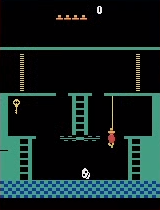
\includegraphics[height=7cm]{./imgs/mz5.png}};
		\begin{scope}[shift=(frame.north west),
				x={(frame.north east)}, y={(frame.south west)}]
			\draw [region box] \boxstart node (start) [region pos, pos=0.5] {};
			\draw [region box] \boxstairsone node (stairs1) [region pos, pos=0.5] {};
		\end{scope}
		\begin{scope}[shift=(frame.south west),
				x={(frame.south east)}, y={(frame.north west)}]
			% Arrows
			\path [path arrow] (start.east) .. controls +(0.05,0) .. (0.7, 0.47);
			\path [path arrow] (0.7, 0.47) .. controls +(0.1,0) .. (stairs1.north);
			\path [path arrow] (stairs1.north west) .. controls
				+(-0.05,0.05) and (0.75, 0.40) .. (0.7, 0.35);
			\path [path arrow] let \p1 = (start.south) in
				(0.7, 0.35) .. controls +(0,0.05) and ($(\x1, 0.45)+(0.05,0)$)
				.. (\x1, 0.40);
			\path [path arrow] let \p1 = (start.south) in
				(\x1, 0.40) -- (start.south);
		\end{scope}
	\end{tikzpicture}
	\caption{Path followed for the ``start''--``stairs1'' goal.}
	\label{fig:mz-repetitive-goal-path}
\end{figure}


\subsection{Comments}

In this second environment, we've shown how to interleave two processes:
training the RL agent and training the features extractor. We gradually
improved the agent's performance until it had been possible to reach a
satisfactory set of symbols. Then, we used this set of fluents to declare a
non-Markovian task, and we've shown a successful training and play with the
Restraining Bolt.

In this small section, we'll make few observations about these experiments on
the Montezuma's Revenge game. First, we highlight some interesting details:
\begin{description}

	\item [Rare events] Although the symbols represented very simple conditions,
		we requested encoder to recognize very rare events. This has been possible
		thanks to Persistent CD, because it focuses on encoding the input
		distribution, not finding the accurate input reconstruction.

	\item [Long training] Restrained RL agents require longer trainings with
		respect to the agent without the Restraining Bolt. Often, this effect
		isn't caused by the additional parameters that are required. Instead, this
		is needed by the more complex policy that we want to learn. Q-values have
		now a more complex landscape that requires to sample pairs of (input
		images--output values) for each automaton state, because the best action
		can be radically different for each of those. Unfortunately, sampling
		cannot be performed uniformly, since the agent has to reach those state.
		So, rare configurations will slow down the training.

\end{description}

Regarding the necessary improvements to this example:
\begin{description}

	\item [Too many actions] With the same training time, as the number of
		action increases, the quality of the policy decreases, because sampling
		becomes less efficient. 18 distinct and independent actions may be too
		much. Instead, we could try to exploit the fact that some of them are just
		a composition of a smaller group of actions, such as: $\const{Left} +
		\const{Up} + \const{Fire}$.

	\item [Explore the map!] We have all the symbols we need to write a temporal
		specification that asks the agent to reach the key, then leave this first
		room of the game. This would be a more interesting challenge to try.
		Instead, in order to navigate the other rooms of the maze, we would need
		to slightly modify the implementation to remove fixed regions. This idea
		is introduced in Section~\ref{sec:future} of ``\nameref{sec:future}''.

\end{description}

